% Figures and tables, one macro per key used in the problem bank.
% Each is authored at full width; the renderer wraps it in an adjustbox
% so it scales down to whatever column it lands in.

\newcommand{\satfigscale}{0.92}

% ---------------------------------------------------------------- tables
\newcommand{\figtblcylab}{%
  \begin{tabular}{|l|c|c|}\hline
     & Volume (cubic units) \\\hline
    Right circular cylinder A & $600\pi$ \\\hline
    Right circular cylinder B & $4{,}800\pi$ \\\hline
  \end{tabular}}

\newcommand{\figtblcyljk}{%
  \begin{tabular}{|c|c|c|}\hline
    Cylinder & Volume & Surface Area \\\hline
    $A$ & $1{,}296\pi$ & $k\pi$ \\\hline
    $B$ & $162{,}000\pi$ & $j\pi$ \\\hline
  \end{tabular}}

\newcommand{\figtblbacteria}{%
  \begin{tabular}{|c|c|}\hline
    Time (months) & Total Bacteria \\\hline
    $0$ & $250$ \\\hline
    $1$ & $b$ \\\hline
    $2$ & $360$ \\\hline
  \end{tabular}}

\newcommand{\figtblfreqab}{%
  \begin{tabular}{|c|c|c|}\hline
    Value & Data set A frequency & Data set B frequency \\\hline
    $10$ & $2$ & $6$ \\\hline
    $20$ & $3$ & $9$ \\\hline
    $30$ & $1$ & $4$ \\\hline
    $40$ & $2$ & $5$ \\\hline
  \end{tabular}}

\newcommand{\figtblbasketball}{%
  \begin{tabular}{|l|c|}\hline
    Position & Frequency \\\hline
    Point guard & $26$ \\\hline
    Shooting guard & $16$ \\\hline
    Small forward & $11$ \\\hline
    Power forward or center & $35$ \\\hline
  \end{tabular}}

\newcommand{\figtblsamples}{%
  \begin{tabular}{|c|c|c|}\hline
    Sample & Percent in favor & Margin of error \\\hline
    $A$ & $67.83\%$ & $7.8\%$ \\\hline
    $B$ & $72.94\%$ & $4.5\%$ \\\hline
  \end{tabular}}

\newcommand{\figtblgx}{%
  \begin{tabular}{|c|c|}\hline
    $x$ & $g(x)$ \\\hline
    $4$ & $9$ \\\hline
    $2$ & $0$ \\\hline
  \end{tabular}}

\newcommand{\figtblfxquad}{%
  \begin{tabular}{|c|c|}\hline
    $x$ & $f(x)$ \\\hline
    $-9$ & $155$ \\\hline
    $-3$ & $227$ \\\hline
    $3$ & $155$ \\\hline
  \end{tabular}}

\newcommand{\figtblrectsim}{%
  \begin{tabular}{|l|c|c|}\hline
      & Volume (cubic inches) & Surface Area (square inches) \\\hline
    Rectangle $A$ & $4{,}374$ & $1{,}782$ \\\hline
    Rectangle $B$ & $1{,}500{,}282$ & $k$ \\\hline
  \end{tabular}}

% the four answer choices of the smallest-standard-deviation item are
% themselves tables, so they are set here rather than as a choice list.
\newcommand{\figtblfreqchoice}{%
  \newcommand{\ftbl}[5]{\begin{tabular}{|c|c|}\hline Value & Frequency \\\hline
    $2$ & $##1$ \\\hline $10$ & $##2$ \\\hline $15$ & $##3$ \\\hline
    $20$ & $##4$ \\\hline $24$ & $##5$ \\\hline\end{tabular}}%
  \begin{tabular}{@{}cccc@{}}
    A) & B) & C) & D) \\[2pt]
    \ftbl{1}{5}{3}{5}{1} & \ftbl{0}{20}{25}{20}{0} &
    \ftbl{100}{50}{25}{0}{25} & \ftbl{45}{55}{65}{75}{85} \\
  \end{tabular}}

% --------------------------------------------------------------- figures
\newcommand{\figcircleoabc}{%
  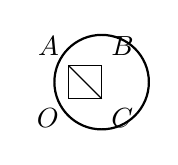
\begin{tikzpicture}[scale=0.05]
    \draw[thick] (0,0) circle (12);
    \coordinate (O) at (-8.4,-4.2); \coordinate (B) at (0,4.2);
    \coordinate (A) at (-8.4,4.2);  \coordinate (C) at (0,-4.2);
    \draw (O)--(A)--(B)--(C)--cycle; \draw (A)--(C);
    \node[above left] at (A) {$A$}; \node[above right] at (B) {$B$};
    \node[below left] at (O) {$O$}; \node[below right] at (C) {$C$};
  \end{tikzpicture}}

\newcommand{\figparallelpqr}{%
  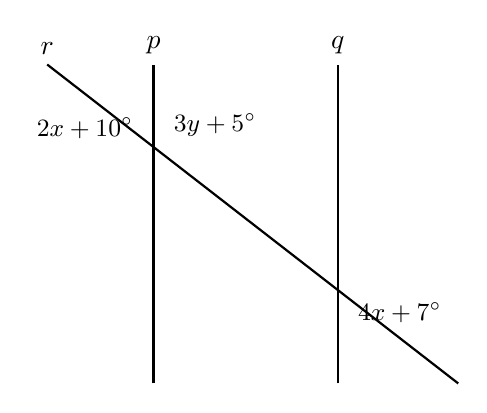
\begin{tikzpicture}[scale=0.9]
    \draw[thick] (0,-2.6)--(0,1.9) node[above] {$p$};
    \draw[thick] (2.6,-2.6)--(2.6,1.9) node[above] {$q$};
    \draw[thick] (-1.5,1.9) node[above] {$r$} --(4.3,-2.6);
    \node[left]  at (-0.15,1.0) {\small $2x+10^\circ$};
    \node[right] at (0.15,1.05) {\small $3y+5^\circ$};
    \node[right] at (2.75,-1.6) {\small $4x+7^\circ$};
  \end{tikzpicture}}

\newcommand{\figbowtie}{%
  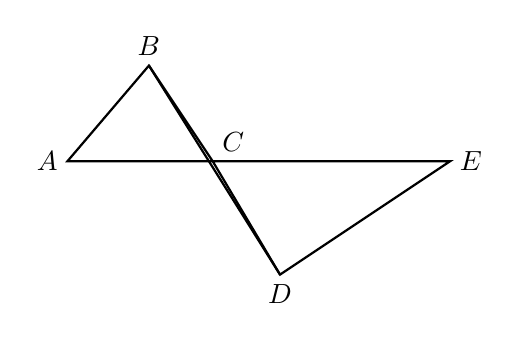
\begin{tikzpicture}[scale=0.9]
    \coordinate (A) at (0,0);   \coordinate (E) at (5.4,0);
    \coordinate (B) at (1.15,1.35); \coordinate (D) at (3.0,-1.6);
    \coordinate (C) at (2.05,0);
    \draw[thick] (A)--(B)--(C)--cycle; \draw[thick] (C)--(D)--(E)--cycle;
    \draw[thick] (A)--(E); \draw[thick] (B)--(D);
    \node[left] at (A) {$A$}; \node[above] at (B) {$B$};
    \node[above right] at (C) {$C$}; \node[below] at (D) {$D$};
    \node[right] at (E) {$E$};
  \end{tikzpicture}}

\newcommand{\figtrianglepqrs}{%
  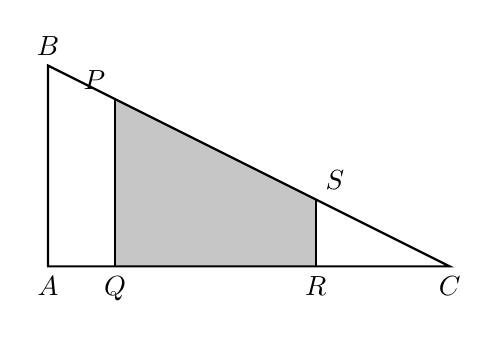
\begin{tikzpicture}[scale=0.85]
    \coordinate (A) at (0,0); \coordinate (C) at (6,0); \coordinate (B) at (0,3);
    \coordinate (Q) at (1,0); \coordinate (R) at (4,0);
    \coordinate (P) at (1,2.5); \coordinate (S) at (4,1);
    \fill[gray!45] (Q)--(P)--(S)--(R)--cycle;
    \draw[thick] (A)--(B)--(C)--cycle;
    \draw[thick] (Q)--(P); \draw[thick] (R)--(S);
    \node[below] at (A) {$A$}; \node[below] at (Q) {$Q$};
    \node[below] at (R) {$R$}; \node[below] at (C) {$C$};
    \node[above] at (B) {$B$}; \node[above left] at (P) {$P$};
    \node[above right] at (S) {$S$};
  \end{tikzpicture}}

\newcommand{\figlineg}{%
  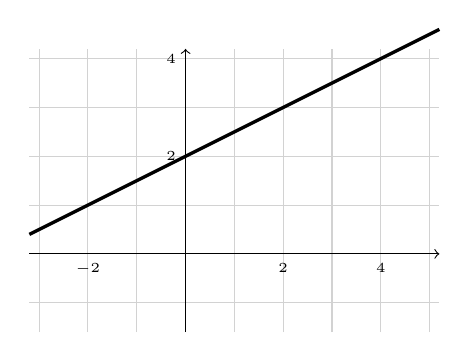
\begin{tikzpicture}[scale=0.62]
    \draw[gray!35,step=1] (-3.2,-1.6) grid (5.2,4.2);
    \draw[->] (-3.2,0)--(5.2,0); \draw[->] (0,-1.6)--(0,4.2);
    \foreach \x in {-2,2,4} \node[below,font=\tiny] at (\x,0) {$\x$};
    \foreach \y in {2,4} \node[left,font=\tiny] at (0,\y) {$\y$};
    \draw[very thick] (-3.2,0.4)--(5.2,4.6);
  \end{tikzpicture}}

\newcommand{\fignestedrect}{%
  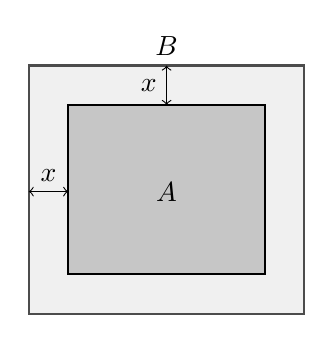
\begin{tikzpicture}[scale=0.5]
    \fill[gray!12] (0,0) rectangle (7,6.3);
    \draw[thick,black!70] (0,0) rectangle (7,6.3);
    \fill[gray!45] (1,1) rectangle (6,5.3);
    \draw[thick] (1,1) rectangle (6,5.3);
    \node[above] at (3.5,6.3) {$B$}; \node at (3.5,3.1) {$A$};
    \draw[<->] (3.5,5.3)--(3.5,6.3) node[midway,left] {$x$};
    \draw[<->] (0,3.1)--(1,3.1) node[midway,above] {$x$};
  \end{tikzpicture}}

\newcommand{\figrighttrisixty}{%
  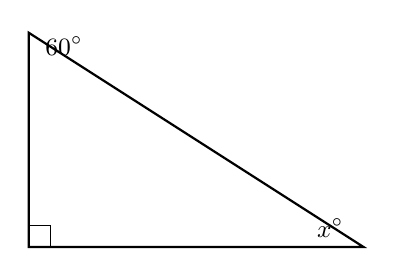
\begin{tikzpicture}[scale=0.85]
    \draw[thick] (0,0)--(0,3.2)--(5,0)--cycle;
    \draw (0,0) rectangle (0.32,0.32);
    \node[right] at (0.1,3.0) {\small $60^\circ$};
    \node[left]  at (4.85,0.28) {\small $x^\circ$};
  \end{tikzpicture}}

\newcommand{\figparallelab}{%
  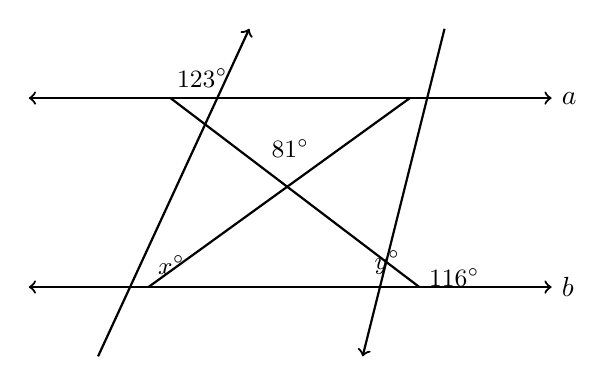
\begin{tikzpicture}[scale=0.8]
    \draw[thick,<->] (-0.9,3)--(7.4,3) node[right] {$a$};
    \draw[thick,<->] (-0.9,0)--(7.4,0) node[right] {$b$};
    \draw[thick,->] (0.2,-1.1)--(2.6,4.1);
    \draw[thick,->] (5.7,4.1)--(4.4,-1.1);
    \draw[thick] (1.35,3)--(5.3,0); \draw[thick] (1.0,0)--(5.15,3);
    \node[above right] at (1.3,3.02) {\small $123^\circ$};
    \node[below right] at (2.8,2.5) {\small $81^\circ$};
    \node[above right] at (1.0,0.05) {\small $x^\circ$};
    \node[above left]  at (5.15,0.05) {\small $y^\circ$};
    \node[right] at (5.3,0.15) {\small $116^\circ$};
  \end{tikzpicture}}

\newcommand{\figcircleabcd}{%
  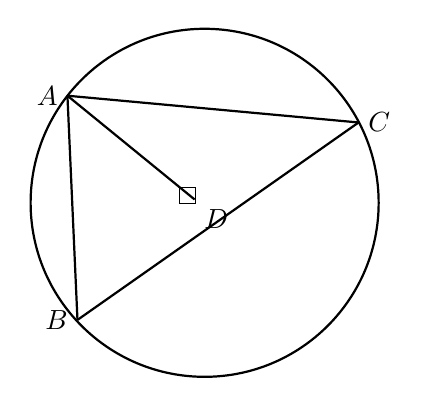
\begin{tikzpicture}[scale=0.85]
    \draw[thick] (0,0) circle (2.6);
    \coordinate (A) at (-2.05,1.6); \coordinate (C) at (2.3,1.2);
    \coordinate (B) at (-1.9,-1.75); \coordinate (D) at (-0.15,0.05);
    \draw[thick] (A)--(C); \draw[thick] (A)--(B); \draw[thick] (B)--(C);
    \draw[thick] (A)--(D);
    \draw (D)++(-0.22,-0.06) rectangle ++(0.24,0.24);
    \node[left] at (A) {$A$}; \node[right] at (C) {$C$};
    \node[left] at (B) {$B$}; \node[below right] at (D) {$D$};
  \end{tikzpicture}}

\newcommand{\figparallelabcde}{%
  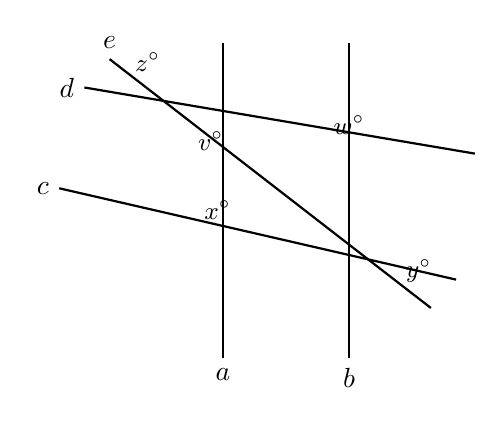
\begin{tikzpicture}[scale=0.8]
    \draw[thick] (1.6,-2.4)--(1.6,2.6) node[below=2pt,anchor=north] {}; \node[below] at (1.6,-2.4) {$a$};
    \draw[thick] (3.6,-2.4)--(3.6,2.6); \node[below] at (3.6,-2.4) {$b$};
    \draw[thick] (-0.6,1.9) node[left] {$d$} --(5.6,0.85);
    \draw[thick] (-0.2,2.35) node[above] {$e$} --(4.9,-1.6);
    \draw[thick] (-1.0,0.3) node[left] {$c$} --(5.3,-1.15);
    \node[above right] at (0.05,2.0) {\small $z^\circ$};
    \node[below right] at (1.05,1.35) {\small $v^\circ$};
    \node[above right] at (3.2,1.0) {\small $w^\circ$};
    \node[above right] at (1.15,-0.35) {\small $x^\circ$};
    \node[above right] at (4.35,-1.35) {\small $y^\circ$};
  \end{tikzpicture}}

\newcommand{\figlinesabk}{%
  \begin{tikzpicture}[scale=0.85]
    \draw[thick] (-0.6,2.2)--(5.6,2.2) node[right] {}; \node[left] at (-0.6,2.2) {$a$};
    \draw[thick] (-0.6,0)--(5.6,0); \node[left] at (-0.6,0) {$b$};
    \draw[thick] (0.6,-1.1)--(3.6,3.4) node[above] {$k$};
    \node[above left]  at (2.35,2.25) {\small $x$};
    \node[above right] at (2.45,2.25) {\small $y$};
    \node[above left]  at (1.05,0.05) {\small $z$};
  \end{tikzpicture}}

\newcommand{\figcirclearc}{%
  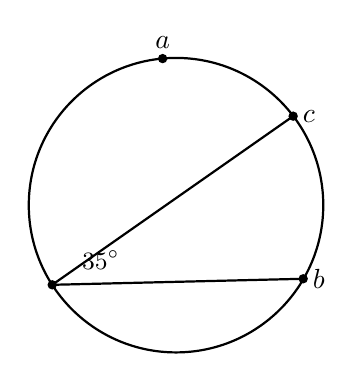
\begin{tikzpicture}[scale=0.85]
    \draw[thick] (0,0) circle (2.2);
    \coordinate (a) at (-0.2,2.19); \coordinate (c) at (1.75,1.33);
    \coordinate (b) at (1.9,-1.1);  \coordinate (v) at (-1.85,-1.19);
    \fill (a) circle (2pt); \fill (c) circle (2pt);
    \fill (b) circle (2pt); \fill (v) circle (2pt);
    \draw[thick] (v)--(c); \draw[thick] (v)--(b);
    \node[above] at (a) {$a$}; \node[right] at (c) {$c$}; \node[right] at (b) {$b$};
    \node[above right] at (-1.55,-1.1) {\small $35^\circ$};
  \end{tikzpicture}}

% ------------------------------------- PrepPros Course #2 additions
\newcommand{\figexpdecay}{%
  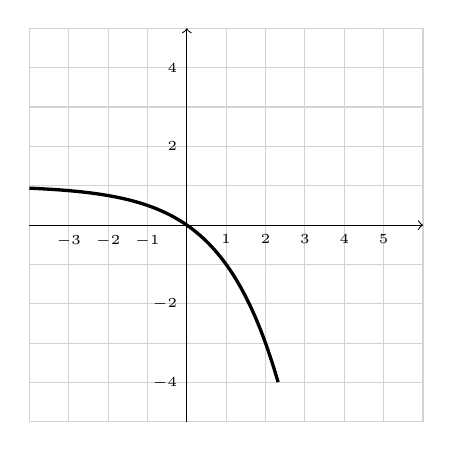
\begin{tikzpicture}[scale=0.5]
    \draw[gray!35,step=1] (-4,-5) grid (6,5);
    \draw[->] (-4,0)--(6,0); \draw[->] (0,-5)--(0,5);
    \foreach \x in {-3,-2,-1,1,2,3,4,5} \node[below,font=\tiny] at (\x,0) {$\x$};
    \foreach \y in {-4,-2,2,4} \node[left,font=\tiny] at (0,\y) {$\y$};
    \draw[very thick,domain=-4:2.32,samples=80] plot (\x,{1-2^(\x)});
  \end{tikzpicture}}

\newcommand{\figcircleabcdii}{%
  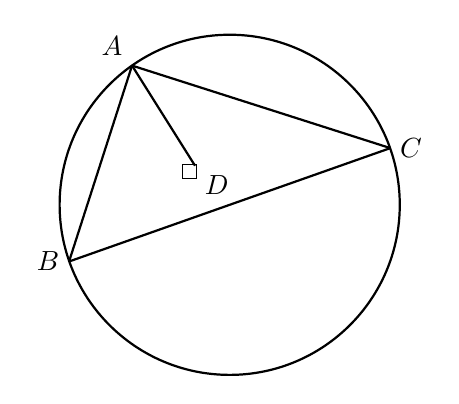
\begin{tikzpicture}[scale=0.8]
    \draw[thick] (0,0) circle (2.7);
    \coordinate (A) at (-1.55,2.21); \coordinate (C) at (2.55,0.9);
    \coordinate (B) at (-2.55,-0.9); \coordinate (D) at (-0.55,0.62);
    \draw[thick] (A)--(C); \draw[thick] (A)--(B); \draw[thick] (B)--(C);
    \draw[thick] (A)--(D);
    \draw (D)++(-0.2,-0.2) rectangle ++(0.22,0.22);
    \node[above left] at (A) {$A$}; \node[right] at (C) {$C$};
    \node[left] at (B) {$B$}; \node[below right] at (D) {$D$};
  \end{tikzpicture}}

\newcommand{\figparallelabcdeii}{%
  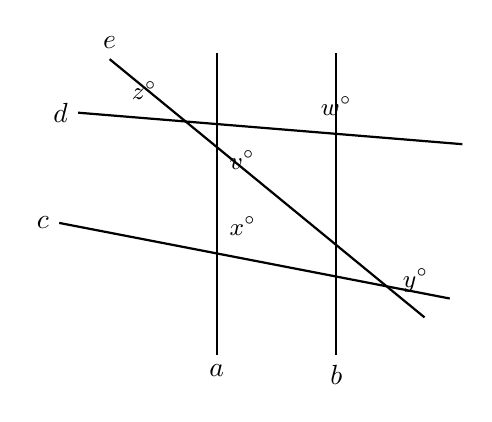
\begin{tikzpicture}[scale=0.8]
    \draw[thick] (1.5,-2.3)--(1.5,2.5); \node[below] at (1.5,-2.3) {$a$};
    \draw[thick] (3.4,-2.3)--(3.4,2.5); \node[below] at (3.4,-2.3) {$b$};
    \draw[thick] (-0.7,1.55) node[left] {$d$} --(5.4,1.05);
    \draw[thick] (-0.2,2.4) node[above] {$e$} --(4.8,-1.7);
    \draw[thick] (-1.0,-0.2) node[left] {$c$} --(5.2,-1.4);
    \node[above right] at (0.0,1.6) {\small $z^\circ$};
    \node[below right] at (1.55,1.1) {\small $v^\circ$};
    \node[above right] at (3.0,1.35) {\small $w^\circ$};
    \node[above right] at (1.55,-0.55) {\small $x^\circ$};
    \node[above right] at (4.3,-1.45) {\small $y^\circ$};
  \end{tikzpicture}}

\newcommand{\figbowtieii}{%
  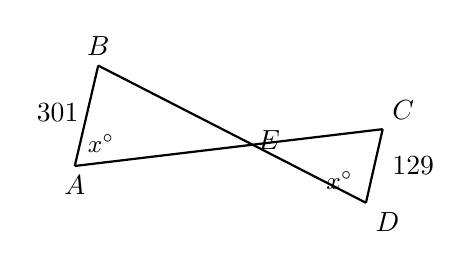
\begin{tikzpicture}[scale=0.85]
    \coordinate (A) at (0,0); \coordinate (B) at (0.35,1.5);
    \coordinate (E) at (2.9,0.1); \coordinate (C) at (4.6,0.55);
    \coordinate (D) at (4.35,-0.55);
    \draw[thick] (A)--(B); \draw[thick] (B)--(D); \draw[thick] (A)--(C);
    \draw[thick] (C)--(D);
    \node[below] at (A) {$A$}; \node[above] at (B) {$B$};
    \node[above] at (E) {$E$}; \node[above right] at (C) {$C$};
    \node[below right] at (D) {$D$};
    \node[left] at (0.2,0.8) {$301$}; \node[right] at (4.6,0.0) {$129$};
    \node[above right] at (0.05,0.05) {\small $x^\circ$};
    \node[above left] at (4.3,-0.5) {\small $x^\circ$};
  \end{tikzpicture}}

\newcommand{\figbowtieiii}{%
  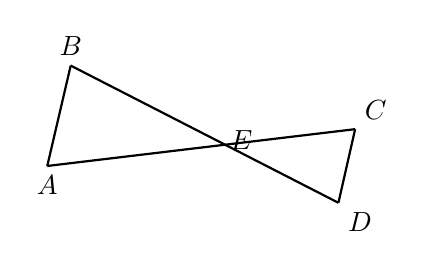
\begin{tikzpicture}[scale=0.85]
    \coordinate (A) at (0,0); \coordinate (B) at (0.35,1.5);
    \coordinate (E) at (2.9,0.1); \coordinate (C) at (4.6,0.55);
    \coordinate (D) at (4.35,-0.55);
    \draw[thick] (A)--(B); \draw[thick] (B)--(D); \draw[thick] (A)--(C);
    \draw[thick] (C)--(D);
    \node[below] at (A) {$A$}; \node[above] at (B) {$B$};
    \node[above] at (E) {$E$}; \node[above right] at (C) {$C$};
    \node[below right] at (D) {$D$};
  \end{tikzpicture}}

\newcommand{\figlineaii}{%
  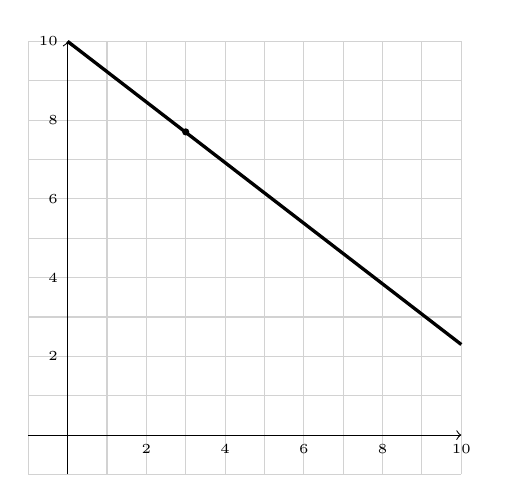
\begin{tikzpicture}[scale=0.5]
    \draw[gray!35,step=1] (-1,-1) grid (10,10);
    \draw[->] (-1,0)--(10,0); \draw[->] (0,-1)--(0,10);
    \foreach \x in {2,4,6,8,10} \node[below,font=\tiny] at (\x,0) {$\x$};
    \foreach \y in {2,4,6,8,10} \node[left,font=\tiny] at (0,\y) {$\y$};
    \draw[very thick] (0,10)--(10,2.3);
    \fill (3,7.7) circle (2.6pt);
  \end{tikzpicture}}

\newcommand{\figrighttrixyz}{%
  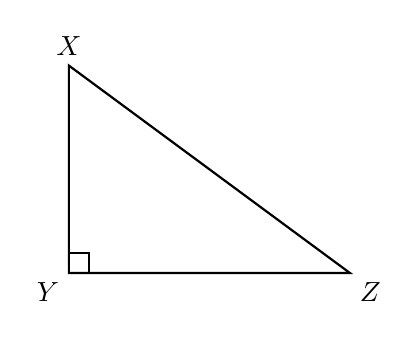
\begin{tikzpicture}[scale=0.85]
    \draw[thick] (0,3.1)--(0,0)--(4.2,0)--cycle;
    \draw (0,0) rectangle (0.3,0.3);
    \node[above] at (0,3.1) {$X$}; \node[below left] at (0,0) {$Y$};
    \node[below right] at (4.2,0) {$Z$};
  \end{tikzpicture}}
